\documentclass{article}
\usepackage{listings}
\usepackage{graphicx}

\title{ASSIGNMENT}
\author{PASUNUTI BHAVANA}
\date{24-05-2019}

\begin{document}
\maketitle
\newpage
\section{QUESTION}
\subsection{DESIGN A 4 BIT UP COUNTER WITH JK FLIPFLOP AND DISPLAY THE OUTPUT ON SSD USING 7447 IC}


\title\underline{LOGIC FUNCTION}
\lstinputlisting{codes/jklogic.c}

\begin{figure}

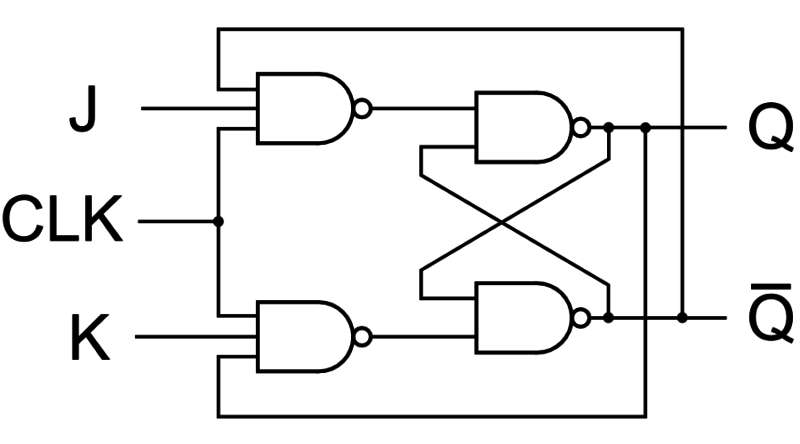
\includegraphics[scale=0.5]{images/logic.png}
\caption{JK flipflop circuit}

\end{figure}
\begin{figure}

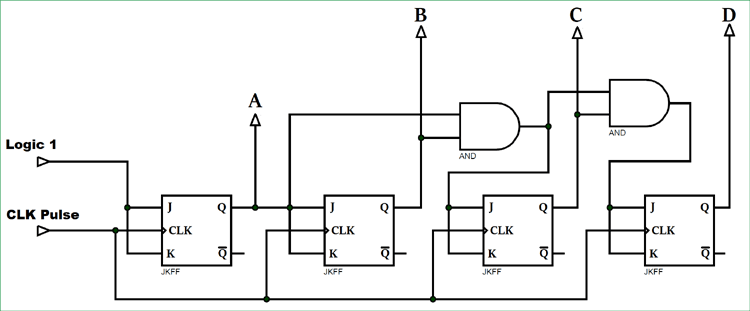
\includegraphics[scale=0.5]{images/counter.png}
\caption{Counter Circuit}
\end{figure}
\newpage
\title\underline{PROGRAM}
\lstinputlisting{codes/jk4bitup.ino}
\newpage
\subsection{DESIGN A 4 BIT DOWN COUNTER WITH JK FLIPFLOP AND DISPLAY THE OUTPUT ON SSD USING 7447 IC}

\title\underline{PROGRAM}
\lstinputlisting{codes/jk4bitdown.ino}

\end{document}